\section{实验结果分析}
算法源码参见附录\ref{appendix}, 本项目报告及实验结果开源: 
\url{https://github.com/WANGH950/Statistical-Machine-Learning/tree/main/2ND}.

\subsection{朴素贝叶斯模型结果分析}
葡萄酒品种分类数据集中的13个特征都为连续型数据, 因此我们在模型训练时保存了训练集特征的最小值和最大值, 并将所有特征值归一化到$[-1,1]$, 确保它们的尺度相同.

由于归一化参数仅通过训练集得到, 用这些参数对测试数据进行归一化后, 其可能会分布到$[-1,1]$以外, 因此我们将 $[-1,1]$ 等距划分为 $S - 2$ 个小区间, 并分别计算了各特征在 $(-\infty,-1), [1,+\infty), [x_k,x_{k+1}), x_k = -1+\frac{2(k-1)}{S-2}, k = 1,2,\cdots S-1$ 个小区间内的条件概率
\begin{equation}
    P_{\lambda}(X^{j}\in S_{jk}|Y = c_k) = \frac{\sum_{i=1}^{N}I(x_{j}\in S_{jk},y_i = c_k) + \lambda}{\sum_{i=1}^{N}I(y_i = c_k) + S\lambda}
\end{equation}
和先验概率
\begin{equation}
    P_{\lambda}(Y = c_k) = \frac{\sum_{i=1}^{N}I(y_i = c_k) + \lambda}{N + K\lambda},
\end{equation}
其中, $S_{jk} = [x_k,x_{k+1}),k = 1,\cdots,S-1, S_{j0} = (-\infty,-1), S_{jS} = [1,+\infty)$, $N$为训练样本数量, $\lambda$ 为Laplacian平滑参数, $K$ 为类别个数.
注意, 为方便起见, 我们将每个特征的区间划分数量设置为同一值 $S$. 

\begin{lstlisting}[caption={朴素贝叶斯模型训练算法部分源码}]
...
for i in range(self.K):
    labels_i = labels == self.full_labels[i]
    self.pre_prob[i] = (labels_i.sum() + self.lamb) / (N + self.K*self.lamb)
    for j in range(self.n):
        self.cond_prob[i,j,0] = 1 / self.S
        for k in range(self.S-1):
            l = -1 + k * delta_x
            r = l + delta_x
            features_ij = features[labels_i[:,0],j]
            features_ijk = features_ij[(features_ij>=l)*(features_ij<r)]
            self.cond_prob[i,j,k+1] = (features_ijk.shape[0] + self.lamb) / (labels_i.sum() + self.S*self.lamb)
...
\end{lstlisting}

我们实例化模型, 训练模型, 并在测试集上测试, 得到了$95.83\%$的准确率.
\subsection{Logistic回归模型结果分析}
我们采用多项逻辑斯谛回归模型
\begin{equation}
    \begin{aligned}
        P(Y = k|x) &= \frac{exp(w_k\cdot x + b_k)}{1 + \sum_{i = 1}^{K-1}exp(w_k\cdot x + b_k)}, k = 1,2,\cdots,K-1\\
        P(Y = K|x) &= \frac{1}{1 + \sum_{i = 1}^{K-1}exp(w_k\cdot x + b_k)}.
    \end{aligned}
\end{equation}
以处理本文的三分类($K=3$)任务. 

为学习模型参数, 我们实现了多类别的负对数似然损失函数
\begin{equation}
    L(\theta) = -\sum_{i=1}^{N}\sum_{k=1}^{K}y_{ik}log(\pi_{\theta_k}(x_i)).
\end{equation}
\begin{lstlisting}
# 负对数似然损失函数
class NLLLoss(nn.Module):
    def __init__(self) -> None:
        super().__init__()
    
    def forward(self,y_pre,y_rel):
        assert y_pre.shape == y_rel.shape
        loss = -torch.log(y_pre)*y_rel
        return torch.sum(loss)
\end{lstlisting}

我们使用小批量梯度下降方法训练数据, 每次在训练数据中均匀随机采样batch条数据进行训练.
我们还在训练模型时将数据的标签进行one-hot编码, 以使用该方法. 
\begin{lstlisting}
index = torch.randint(0,N,[batch_size]) # 随机选取batch条数据
data_i = data_set[index,:]
x_i = data_i[:,:-1].to(torch.float32)
y_i = nn.functional.one_hot(data_i[:,-1].to(torch.int64),num_classes=model.class_num)
\end{lstlisting}
在数据经过线性层以前, 我们先对其进行了批量归一化, 自动学习相应的归一化参数.

我们实例化模型, 选择批处理大小为$20$, 在$1e-3$的学习率下在训练数据上迭代了$2,000$次, 得到了最终的模型.
我们使用训练好的模型在测试集上进行测试, 得到了$97.22\%$的准确率.
该非线性模型效果略好于朴素贝叶斯模型.

\subsection{支持向量机模型结果分析}
我们分别实现了线性和非线性支持向量机模型. 
如图\ref{figure1}, 简单观察数据, 我们可以得到第二个特征和第三个特征以及第二个特征和第四个特征的非线性可分关系.
\begin{figure}[htpb]
    \centering
    \subfigure[第二个特征和第三个特征关于标签$0$和非$0$绘制的散点图]{
		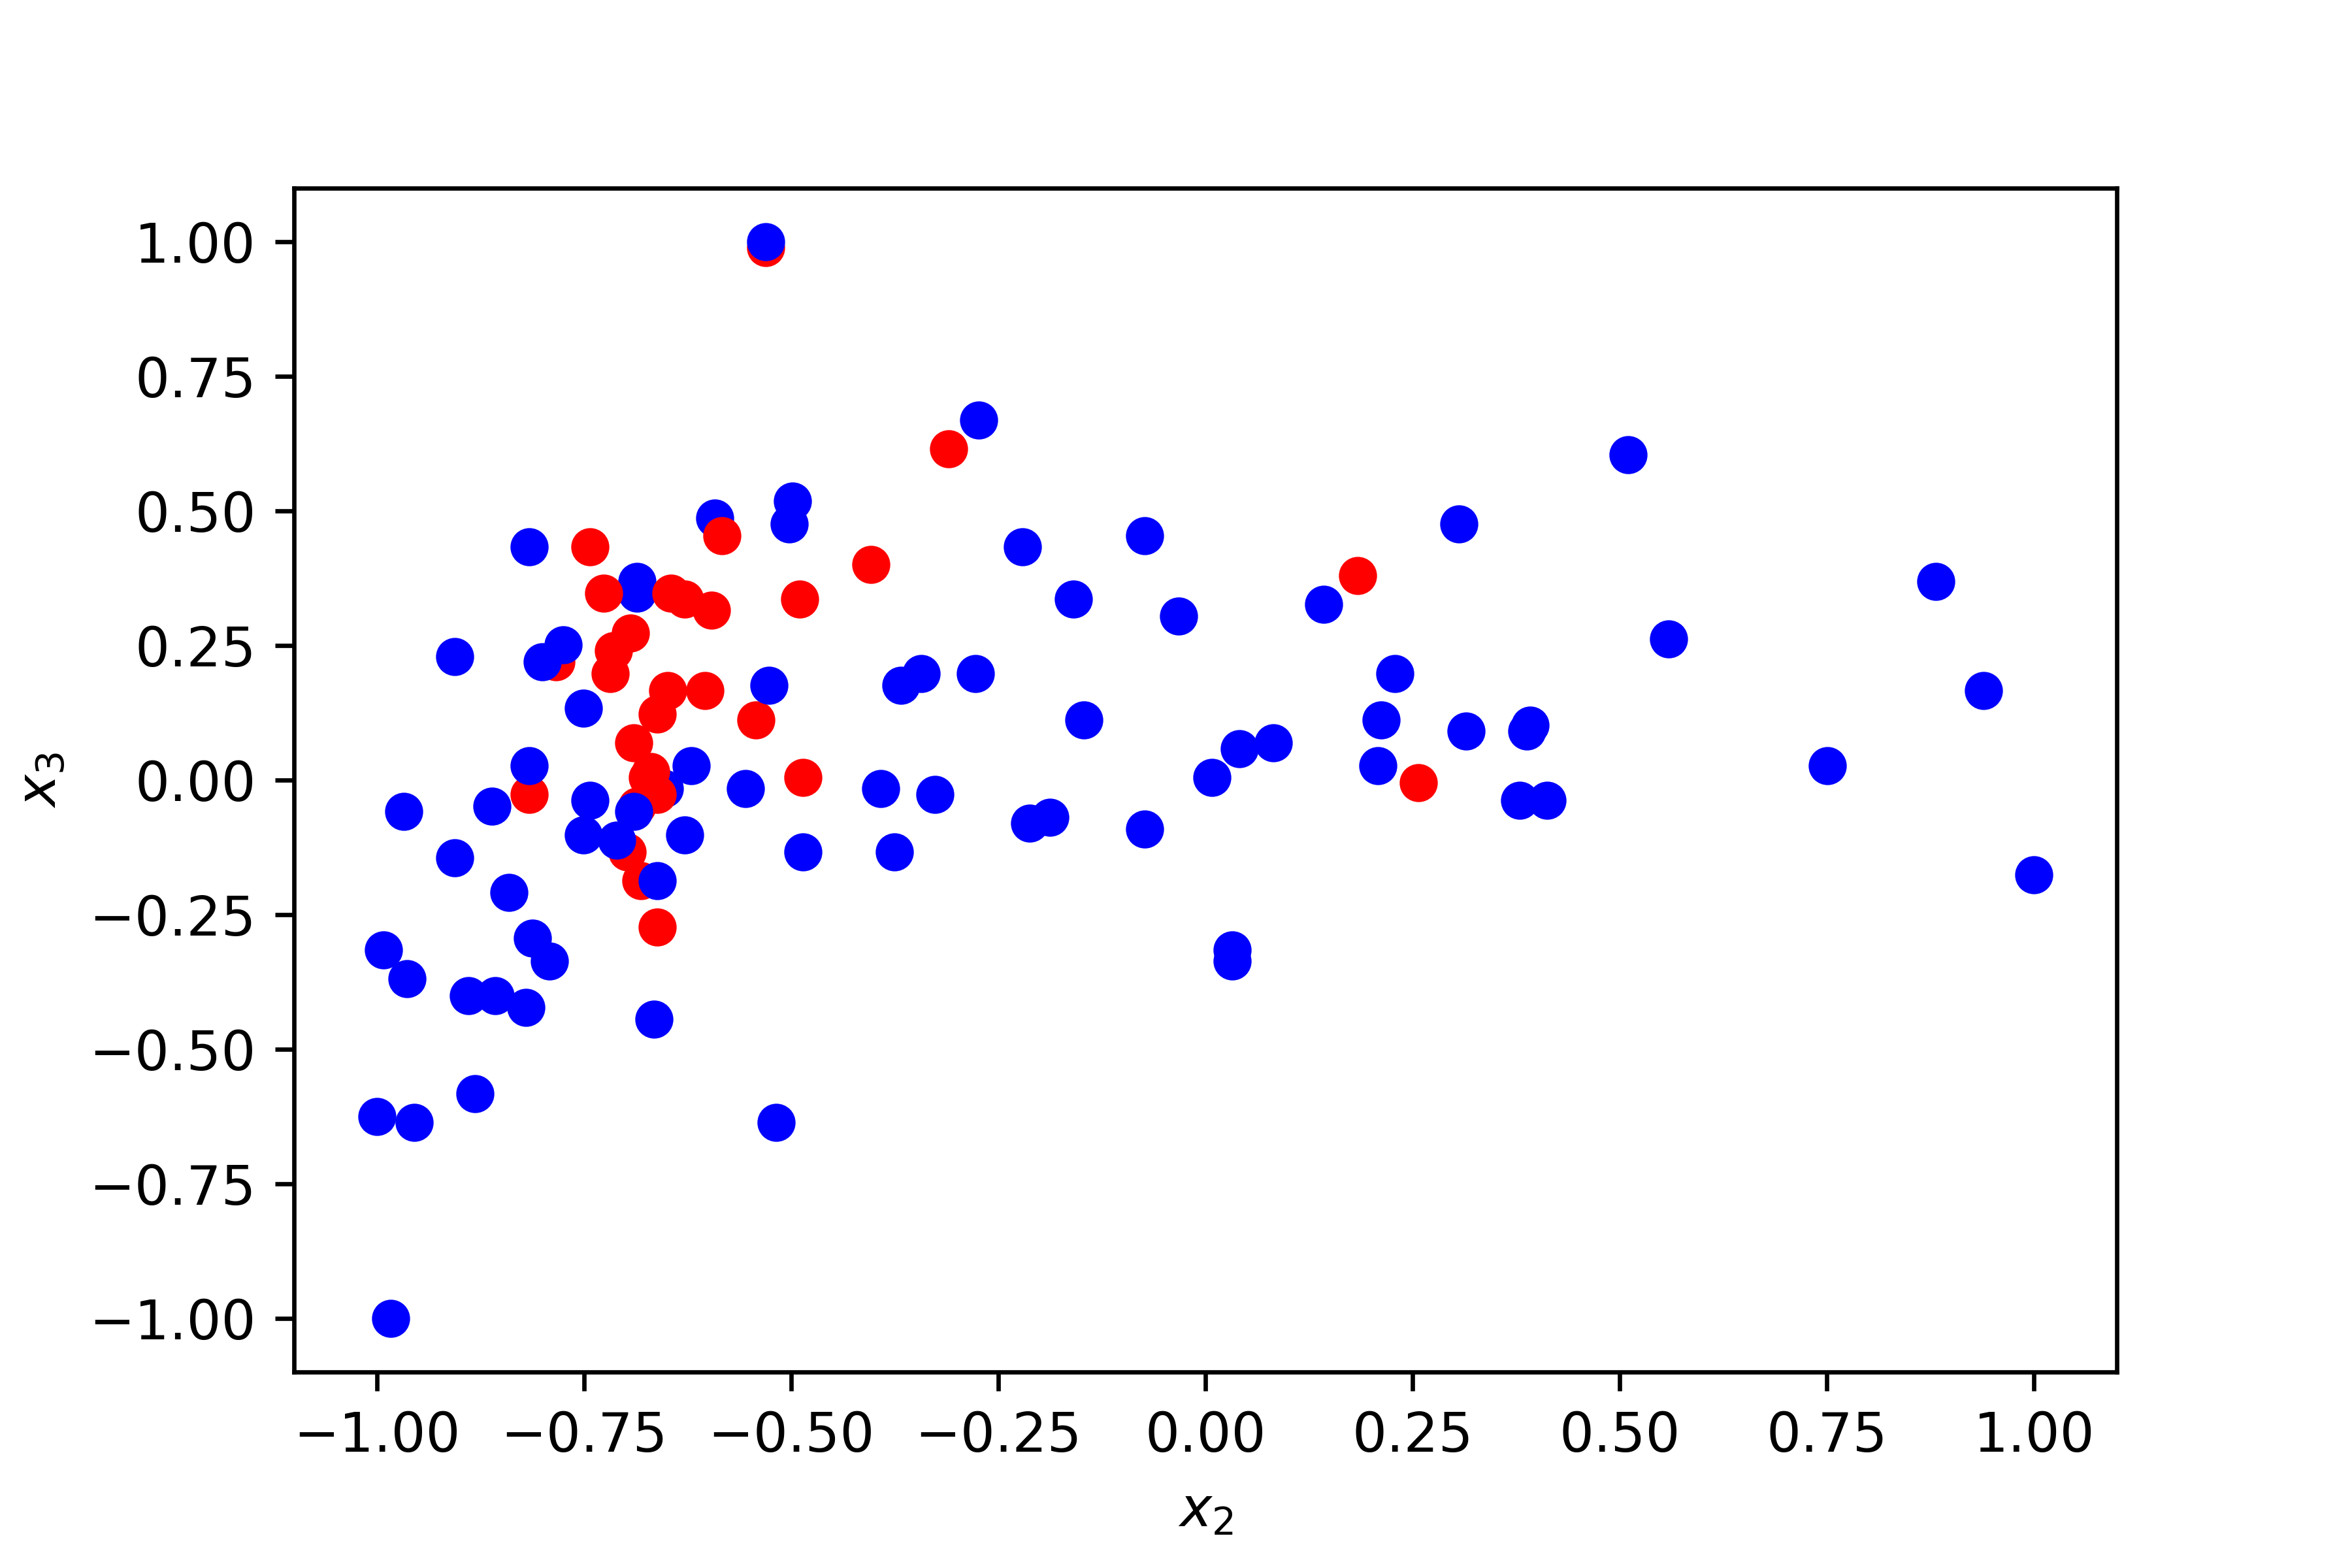
\includegraphics[width=0.48\linewidth]{figure/svm1.png}}
	\subfigure[第二个特征和第四个特征关于标签$0$和非$0$绘制的散点图]{
		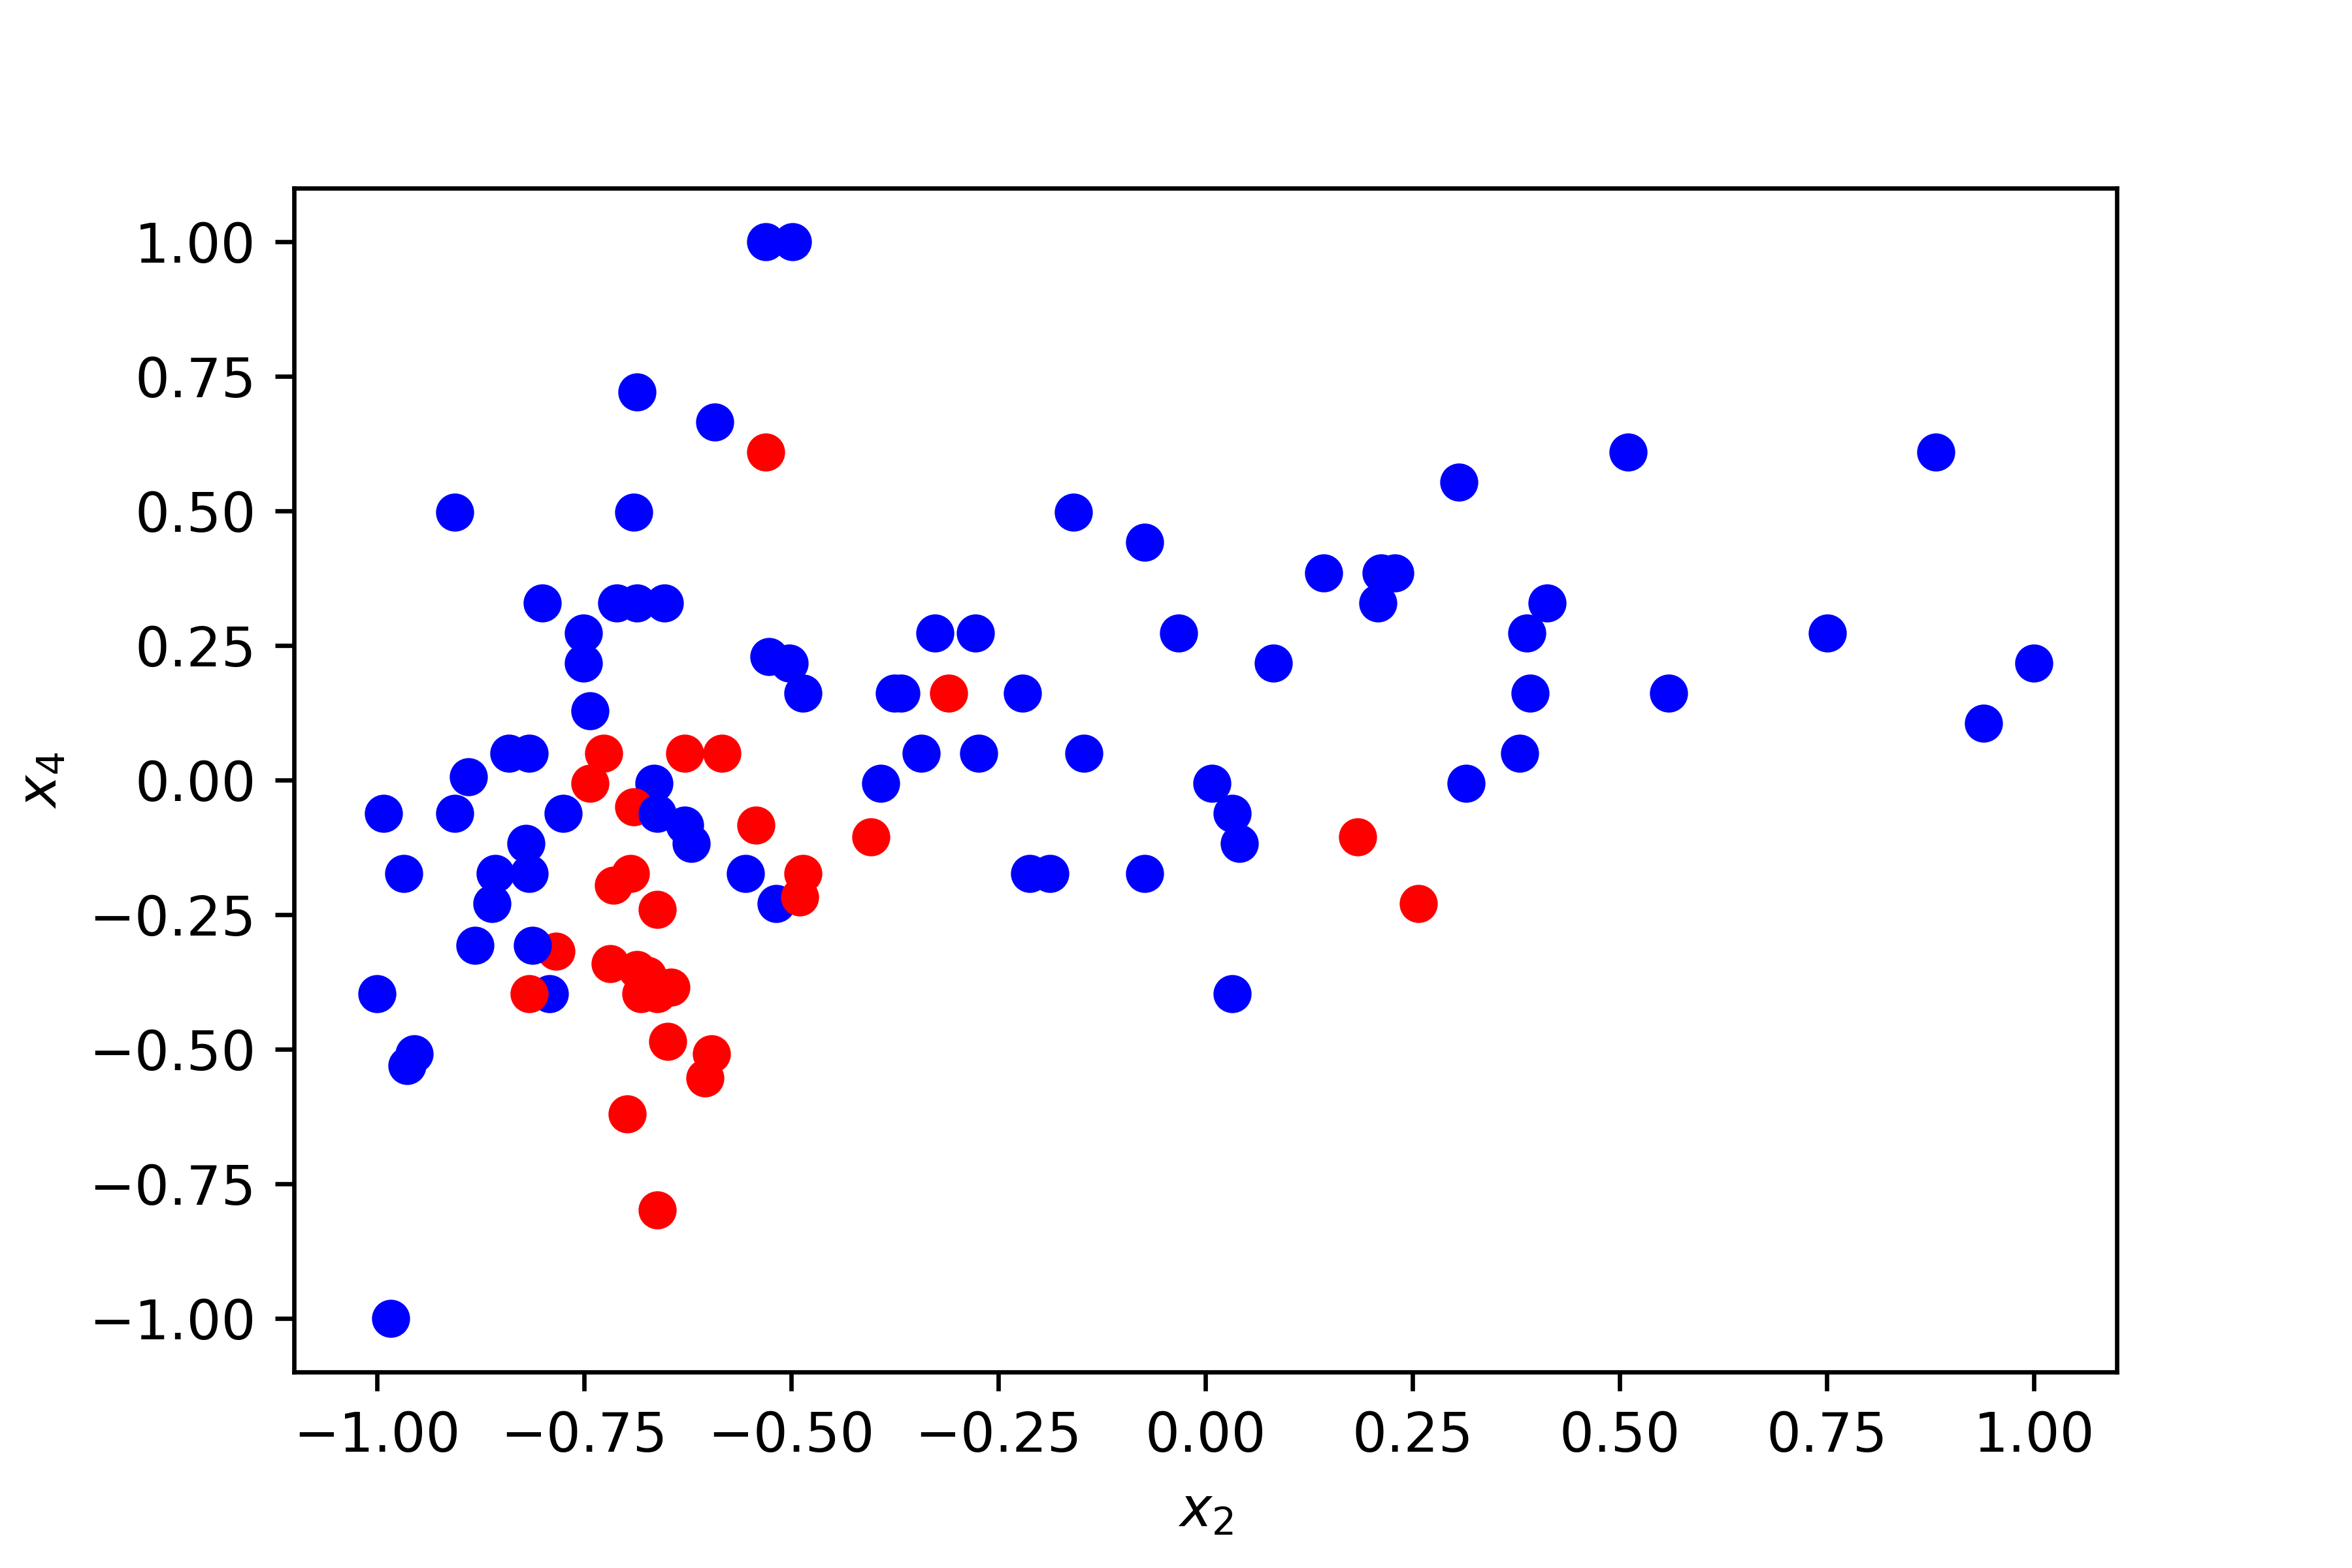
\includegraphics[width=0.48\linewidth]{figure/svm2.png}}
    \caption{非线性可分数据现象图像.}
    \label{figure1}
\end{figure}
因此, 针对非线性支持向量机模型, 我们简单的考虑高斯核函数得到的特征和原始特征结合, 再经过线性分类器对模型进行分类.

我们实现了合页损失函数
\begin{equation}
    L(\theta) = \sum_{i=1}^{N}[1 - y_i(w\cdot x_i + b)]_{+} + \lambda\|w\|^2,
\end{equation}
以用于优化模型, 其中$\theta = \{w,b\}$.
\begin{lstlisting}
# 合页损失函数
class HingeLoss(nn.Module):
    def __init__(self,lamb) -> None:
        super(HingeLoss,self).__init__()
        self.lamb = lamb

    def forward(self,res_pre_linear_values,res_rel,parameters):
        return torch.sum(torch.relu(1 - res_rel*res_pre_linear_values)) + self.lamb*torch.norm(parameters)**2
\end{lstlisting}

由于支持向量机是二分类模型, 我们将原始三分类问题分解为两个二分类问题, 并针对这两类二分类问题各训练了一个模型.

对于线性模型, 我们选取批处理大小$20$, 正则化参数$\lambda = 0.1$, 以$1e-3$的学习率在训练数据上迭代了$2,000$次得到了最终的模型.
对于非线性模型, 我们选择核函数参数$N_s = 20$, 其余参数与线性模型相同.
我们使用训练好的线性模型和非线性模型, 在测试数据上分别得到了$94.44\%,95.83\%$的准确率.
结果表明, 非线性模型的效果略好于线性模型, 但都不如逻辑斯谛回归模型. 

\subsection{神经网络模型结果分析}
多层感知机, 又名全连接前馈神经网络是现在深度学习模型中最基础也是最重要的模型之一.
其通过交替堆叠线性函数和非线性函数(激活函数)而达到对任意函数的万能逼近的作用.
全连接神经网络的结构如图\ref{figure2}.
\begin{figure}[!h]
\centering
\begin{tikzpicture}
  \node[inputNode] (x0) at (0,3) {$x_0$};
  \node[inputNode] (x1) at (0,2) {$x_1$};
  \node[inputNode] (xn) at (0,0) {$x_n$};
  \node[inputNode] (z0) at (2,3) {$\sigma$};
  \node[inputNode] (z1) at (2,2) {$\sigma$};
  \node[inputNode] (zn) at (2,0) {$\sigma$};
  \draw[->] (x0) -- (z0);
  \draw[->] (x0) -- (z1);
  \draw[->] (x0) -- (zn);
  \draw[->] (x1) -- (z0);
  \draw[->] (x1) -- (z1);
  \draw[->] (x1) -- (zn);
  \draw[->] (xn) -- (z0);
  \draw[->] (xn) -- (z1);
  \draw[->] (xn) -- (zn);
  \node[inputNode] (k0) at (4,3) {$\sigma$};
  \node[inputNode] (k1) at (4,2) {$\sigma$};
  \node[inputNode] (kn) at (4,0) {$\sigma$};
  \draw[->] (z0) -- (k0);
  \draw[->] (z0) -- (k1);
  \draw[->] (z0) -- (kn);
  \draw[->] (z1) -- (k0);
  \draw[->] (z1) -- (k1);
  \draw[->] (z1) -- (kn);
  \draw[->] (zn) -- (k0);
  \draw[->] (zn) -- (k1);
  \draw[->] (zn) -- (kn);
  \node[inputNode] (y1) at (6,2.5) {$y_1$};
  \node[inputNode] (y2) at (6,0.5) {$y_m$};
  \node (dots3) at (6,1.5) {$\vdots$};
  \draw[->] (k0) -- (y1);
  \draw[->] (k1) -- (y1);
  \draw[->] (kn) -- (y1);
  \draw[->] (k0) -- (y2);
  \draw[->] (k1) -- (y2);
  \draw[->] (kn) -- (y2);
  \node (dots0) at (0, 1) {$\vdots$};
  \node (dots1) at (2, 1) {$\vdots$};
  \node (dots2) at (4, 1) {$\vdots$};
  \node (inputdim) at (0,-1){$d_{input}$};
  \node (hidden1dim) at (2,-1){$d_{hidden_1}$};
  \node (hidden2dim) at (4,-1){$d_{hidden_2}$};
  \node (outputdim) at (6,-1){$d_{output}$};
\end{tikzpicture}
\caption{\,两层隐藏层的全连接前馈神经网络结构, 其中带箭头的实线表示线性连接, 每条实线都对应一个权重, $\sigma$是非线性函数, 为网络提供非线性因素.}
\label{figure2}
\end{figure}

我们搭建了以Sigmoid Linear Unit(SiLU)
\begin{equation}
    SiLU(x) = \frac{xexp(x)}{1+exp(x)}
\end{equation}
为激活函数的神经网络模型, 并在输出层使用Softmax函数
\begin{equation}
    Softmax(y_i) = \frac{exp(y_i)}{\sum_{i=1}^{K}exp(y_i)}
\end{equation}
归一化.

我们实例化了一个$3$层隐藏层, 每个隐藏层维度为$30$的全连接前馈神经网络.
该模型以$1e-3$的学习率, $20$的批处理大小, 在训练数据上经过$3,000$次迭代, 得到了最终的模型.
模型在测试数据上得到了$97.22\%$的准确率, 精度与逻辑斯谛回归模型相似, 要优于其他模型.